\documentclass{vipweekly}
\usepackage[colorlinks, hyperfootnotes]{hyperref}
\usepackage{hhline}
\usepackage[noadjust]{cite}
\usepackage{listings}
\usepackage{lipsum}
\usepackage{amsfonts}
\usepackage{algorithm} % Pseudo code 작성용
\usepackage{algorithmicx} % Pseudo code 작성용
\usepackage{algpseudocode} % Pseudo code 작성용
\usepackage{xcolor}

\renewcommand{\citedash}{--}

\title{Weekly Report} %% Title은 Weekly Report로 고정합니다.
%% Grade는 아래와 같이 작성합니다. 
\grade{Master's Program} % For 석사과정
\grade{Combined Master's-Doctoral Program} % For 석박사통합과정
\grade{Doctoral Program} % For 박사과정
\grade{U-surf Program} % For 석사과정
\author{Dong-Wook Kim} % 이름은 영문으로 작성합니다. 
\date{\today} % Date는 작성 날짜로 고정합니다. 

\begin{document}
\maketitle
\hypersetup{citecolor=blue}

\section*{Milestones}
\begin{itemize} 
    \item U-surf Program \\
    \begin{itemize}
        \item U-surf Program Due: Jul. 28th\\
    \end{itemize}
\end{itemize}
이번 주에는 
\begin{enumerate}
    \item Custom data를 이용한 InfoNeRF학습
    \item 실험 결과 시각화
    \item InfoNeRF 모델 개선 아이디어 및 실험
    % \begin{itemize}
    %     \item colmap 
    %     \item Backpropagation 구현
    % \end{itemize}
    
\end{enumerate} 
등을 진행하기로 했습니다.


\section{Custom data를 이용한 InfoNeRF학습}

\subsection{Review}

\begin{figure}[h]
    \centering
    \subfloat[input scene1]{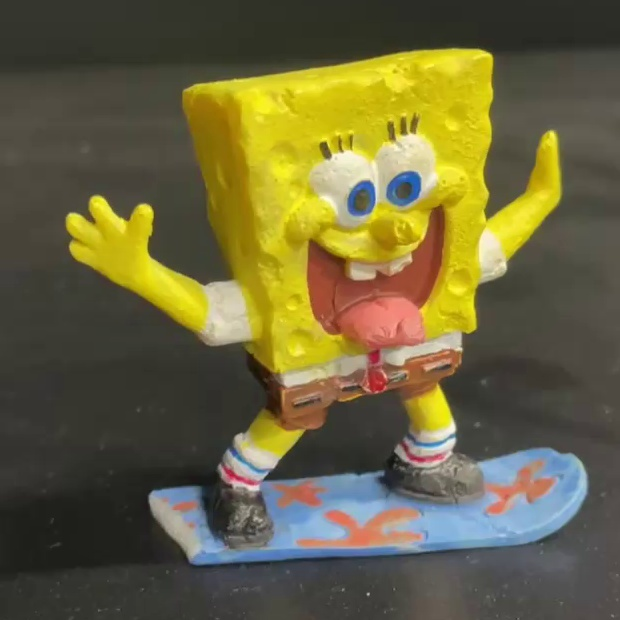
\includegraphics[width=0.25\textwidth]{../images/230724/r_0.png}}\hfill
    \subfloat[input scene2]{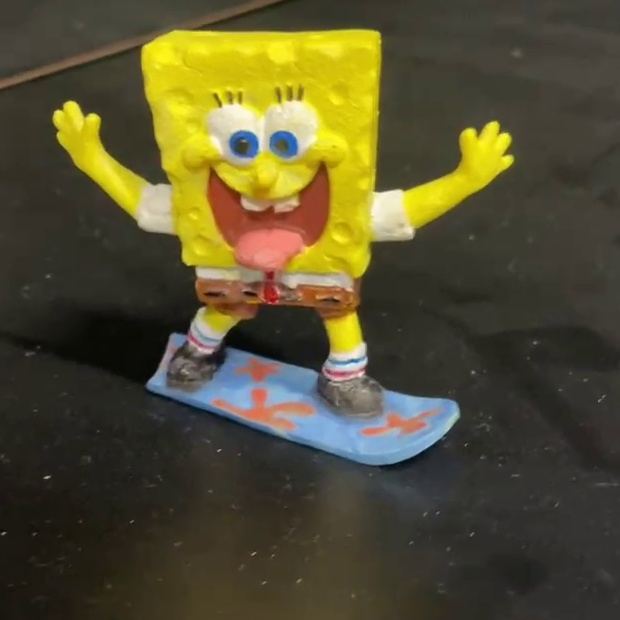
\includegraphics[width=0.25\textwidth]{../images/230724/r_100.png}}\hfill
    \subfloat[input scene3]{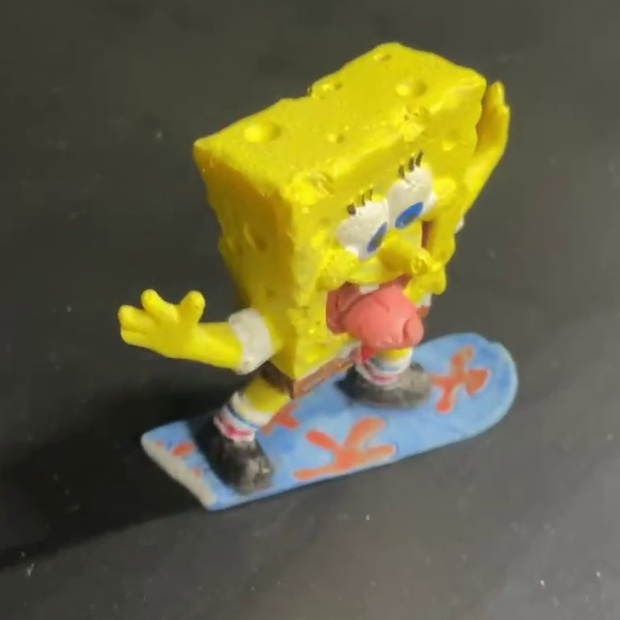
\includegraphics[width=0.25\textwidth]{../images/230724/r_235.png}}\hfill
    \subfloat[input scene4]{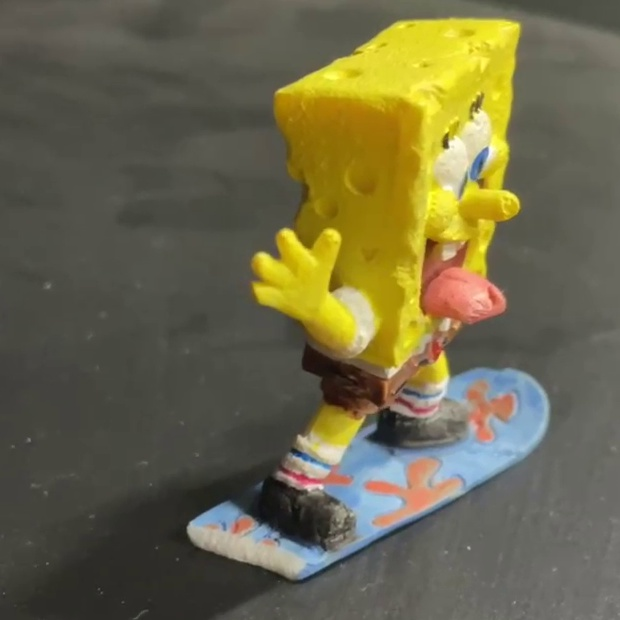
\includegraphics[width=0.25\textwidth]{../images/230724/r_340.png}}\hfill

    \subfloat[rendered image]{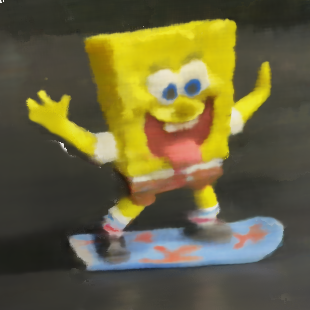
\includegraphics[width=0.15\textwidth]{../images/230717/000_018.png}}\hfill
    \subfloat[rendered image]{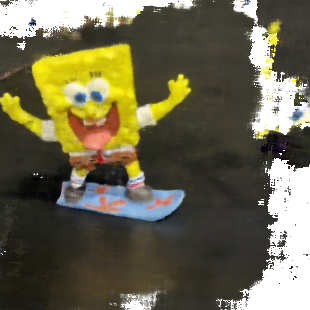
\includegraphics[width=0.15\textwidth]{../images/230717/078_018.png}}\hfill
    \subfloat[rendered image]{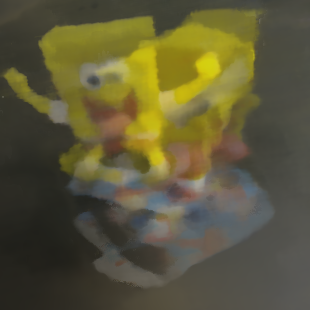
\includegraphics[width=0.15\textwidth]{../images/230717/003_018.png}}\hfill
    \subfloat[depthmap]{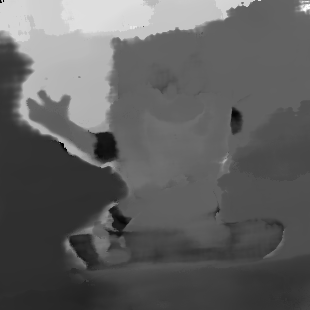
\includegraphics[width=0.15\textwidth]{../images/230717/000_depth_018.png}}\hfill
    \subfloat[depthmap]{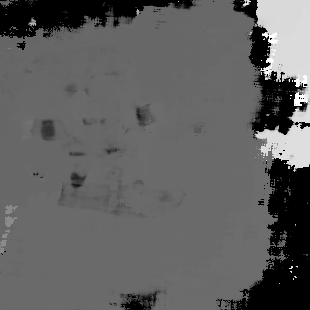
\includegraphics[width=0.15\textwidth]{../images/230717/078_depth_018.png}}\hfill
    \subfloat[depthmap]{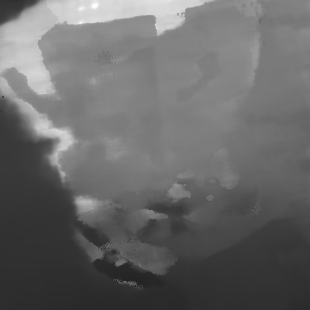
\includegraphics[width=0.15\textwidth]{../images/230717/003_depth_018.png}}\hfill

    \caption{InfoNeRF Results}
    \label{fig:Results}
\end{figure}

지난 시간 \ref{fig:Results}와 같은 결과를 얻고 좋지 못한 결과가 나온 원인으로 아래와 같은 가설을 세웠습니다.

\begin{enumerate}
    \item camera extrinsic의 일부가 잘못되었다.
    \item InfoNeRF의 한계이다. 
    \begin{enumerate}
        \item 좋은 결과가 나왔던 lego dataset에 경우 배경이 없지만 custom data에는 배경이 존재한다.
    \end{enumerate}
\end{enumerate}


위 가설들을 바탕으로 더욱 명확하게 camera extrinsic을 찾고,
코드를 분석하여 논문에서 언급되지 않은 렌더링 옵션 수정하였습니다.

\subsection{Final output of InfoNeRF}

앞선 과정들을 거쳐 최종적으로 얻은 infoNeRF의 결과 이미지는 다음과 같습니다. 

\begin{figure}[h]
    \centering
    \subfloat[rendered scene]{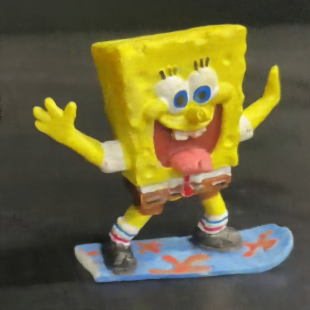
\includegraphics[width=0.25\textwidth]{../images/230724/000.png}}\hfill
    \subfloat[rendered scene]{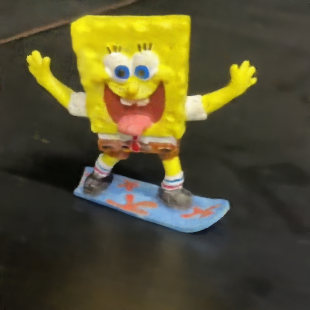
\includegraphics[width=0.25\textwidth]{../images/230724/001.png}}\hfill
    \subfloat[rendered scene]{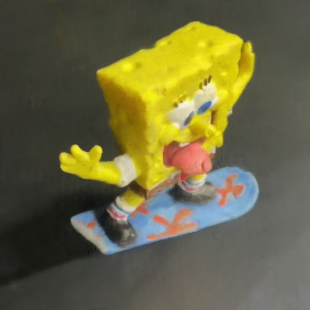
\includegraphics[width=0.25\textwidth]{../images/230724/002.png}}\hfill
    \subfloat[rendered scene]{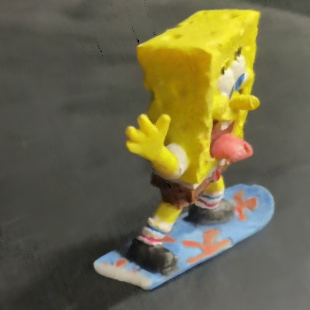
\includegraphics[width=0.25\textwidth]{../images/230724/003.png}}\hfill
    \subfloat[rendered scene]{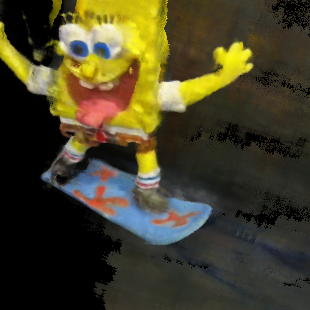
\includegraphics[width=0.25\textwidth]{../images/230724/004.png}}\hfill
    \subfloat[rendered scene]{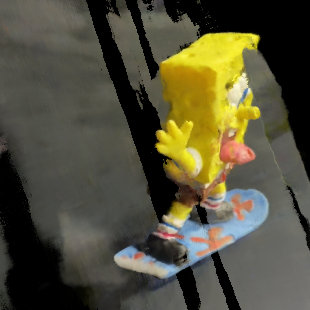
\includegraphics[width=0.25\textwidth]{../images/230724/005.png}}\hfill
    \subfloat[rendered scene]{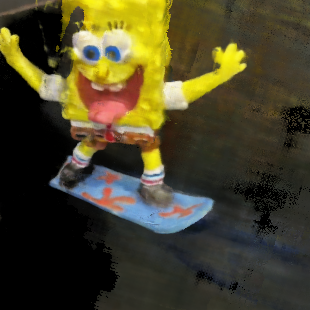
\includegraphics[width=0.25\textwidth]{../images/230724/012.png}}\hfill
    \subfloat[rendered scene]{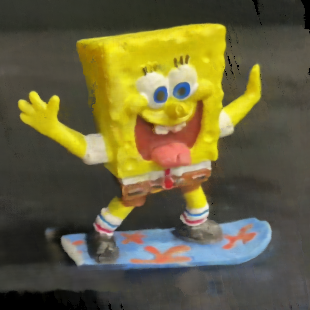
\includegraphics[width=0.25\textwidth]{../images/230724/018.png}}\hfill
    \subfloat[rendered scene]{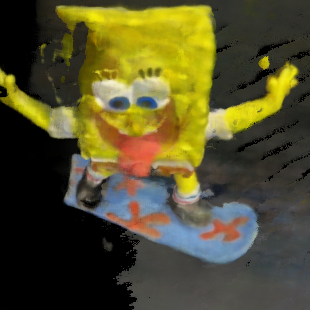
\includegraphics[width=0.25\textwidth]{../images/230724/023.png}}\hfill
    \subfloat[rendered scene]{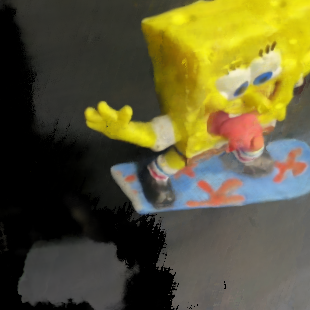
\includegraphics[width=0.25\textwidth]{../images/230724/032.png}}\hfill
    \subfloat[rendered scene]{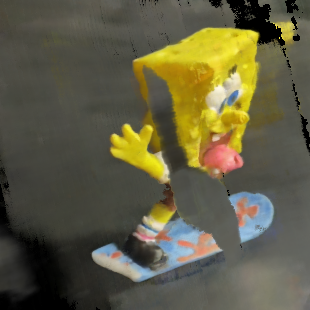
\includegraphics[width=0.25\textwidth]{../images/230724/044.png}}\hfill
    \subfloat[rendered scene]{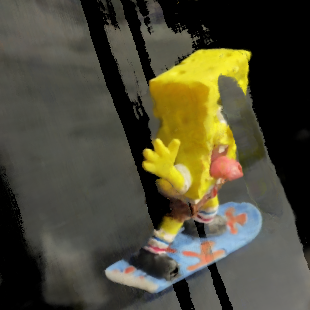
\includegraphics[width=0.25\textwidth]{../images/230724/051.png}}\hfill

    \caption{InfoNeRF Results}
    \label{fig:Results_s}
\end{figure}

이전 결과에 비하여 비약적으로 좋은 결과를 얻을 수 있었다. 
하지만 단순히 rendered scene만으로 point cloud가 잘 형성되었는지 
알기에는 다소 무리가 있기 떄문에 직접 point cloud 를 시각화 하기로 하였다.

\section{실험 결과 시각화}

시각화 tool로는 편의상 'cloud compare'을 사용하였으며, 
기존 모델에서 point cloud 정보를 추가로 수집하였다.

\newpage

\begin{figure}[h]
    \centering
    \subfloat[5000iter point cloud]{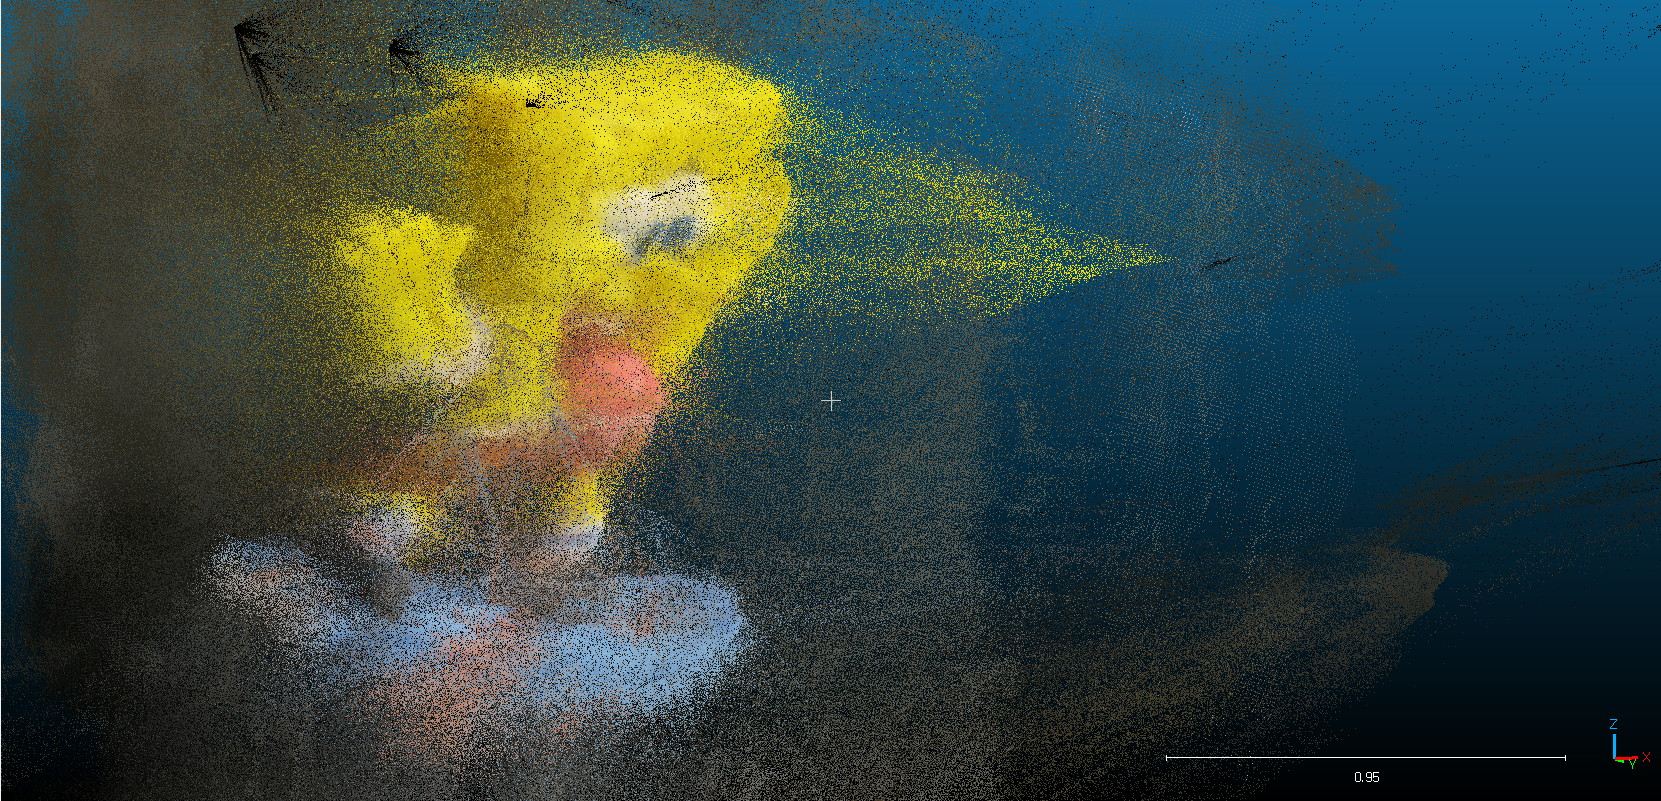
\includegraphics[width=0.5\textwidth]{../images/230724/pc1.png}}\hfill
    \subfloat[30000iter point cloud]{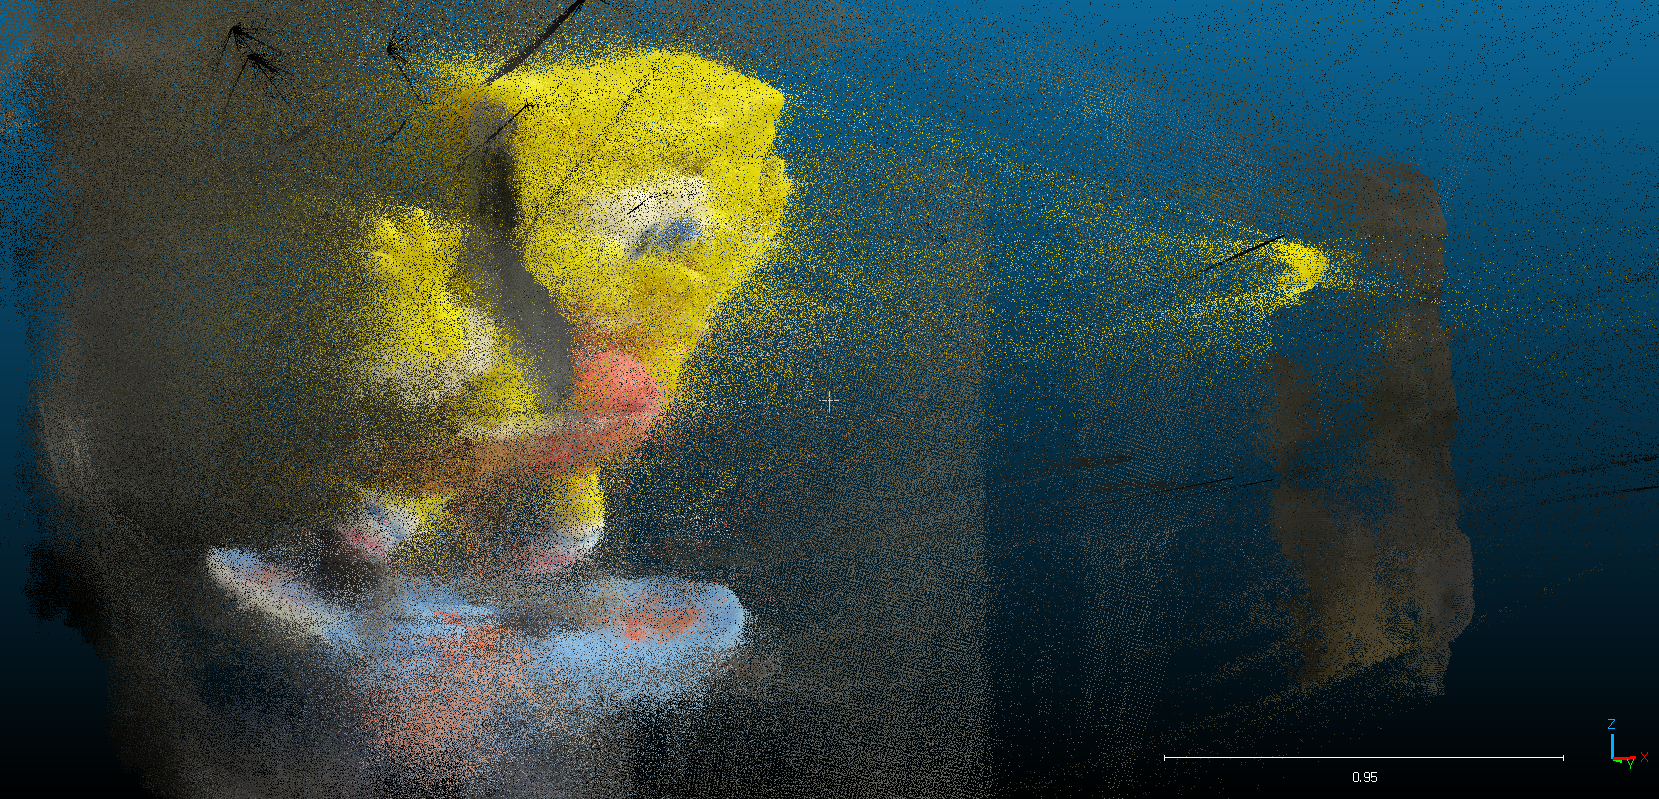
\includegraphics[width=0.5\textwidth]{../images/230724/pc2.png}}\hfill
    \caption{InfoNeRF Results point cloud}
    \label{fig:Results_pc}
\end{figure}

\ref{fig:Results_pc}을 확인해보면 Iteration이 진행될수록 point들이 뭉치는 것을 확인할 수 있다.
하지만 물체 주변이 아닌 위치에 point들이 뭉치는 것을 확인할 수 있다. 
해당 문제를 해결하기 위해 아래와 같은 실험을 진행 혹은 계획 중이다.

\section{InfoNeRF 모델 개선 아이디어 및 실험}

InfoNeRF의 성능향상을 위해 두가지 측면에서의 시도를 해보았다.

\subsection{학습속도 개선} 

이상한 위치에 point 군집이 생기는것을 test scene에 대한 overfitting이 문제로 정의하고
이를 해결하기 위해 아래 논문을 참고하였다.
Dropout Reduces Underfitting(ICML)\cite{Dropout} 논문은 기존 dropout을 
early dropout과 late dropout으로 분리한다.

\begin{figure}[h]
    \centering
    \subfloat{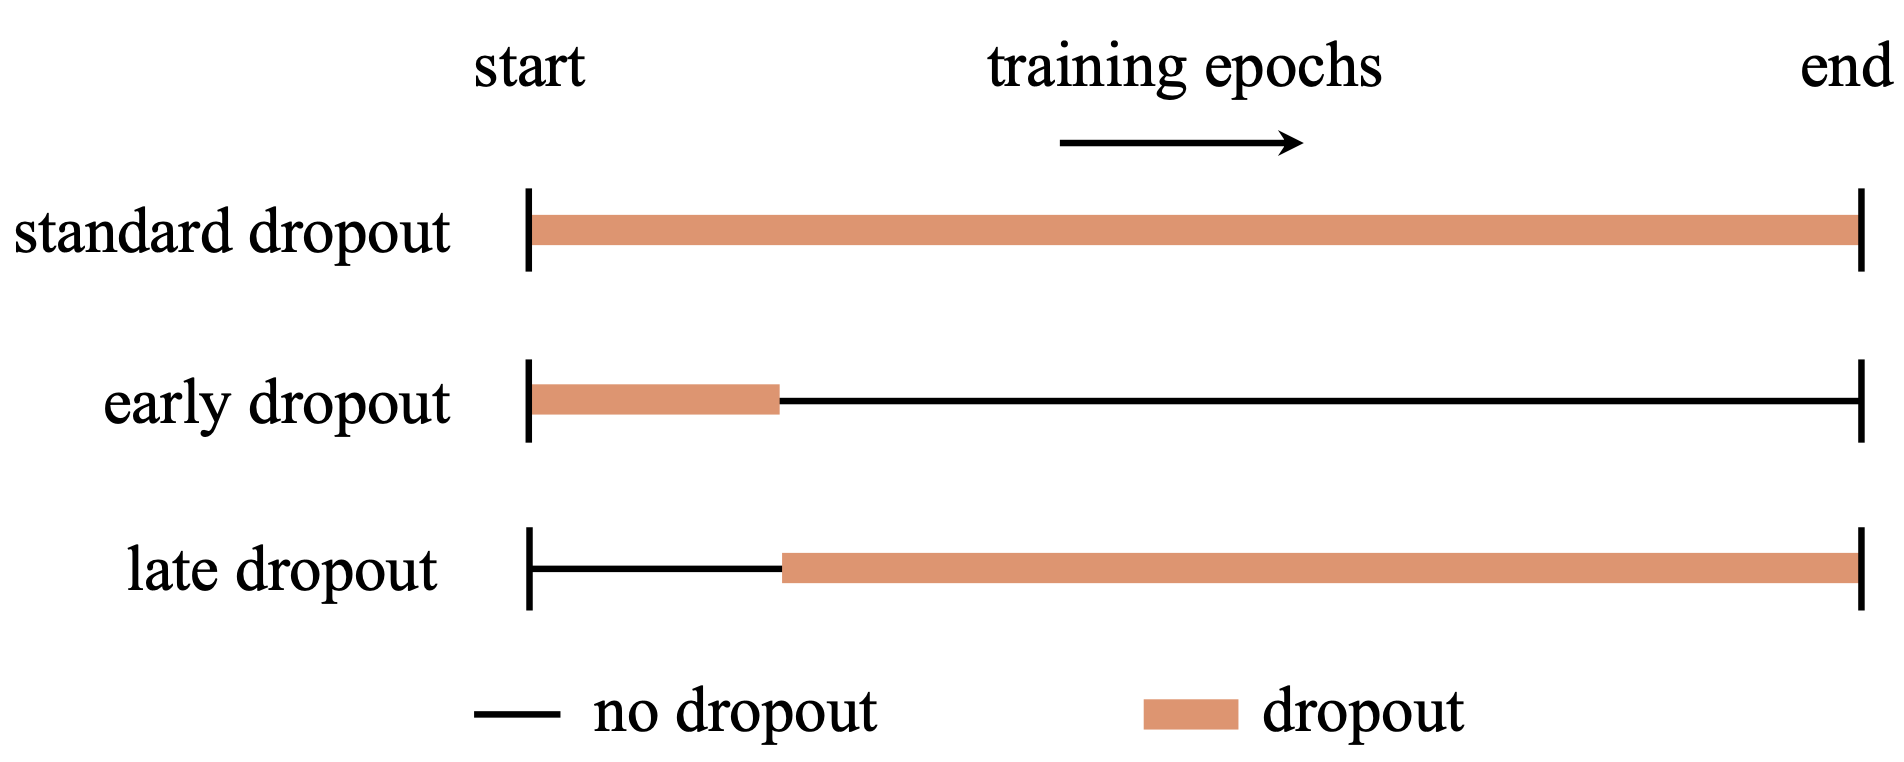
\includegraphics[width=0.8\textwidth]{../images/230724/dropout.png}}\hfill
    \caption{Dropout Reduces Underfitting}
    \label{fig:dropout}
\end{figure}

early dropout은 학습 초기에는 모델이 수렴하는것을 도와주며, late dropout은 학습의 overfitting을 방지함을 주장한다.
해당 구조에 착안하여 기존 InfoNeRF에 early dropout을 적용하여 모델이 적은 Iteration만으로 수렴이 가능할지 실험하였다.



\begin{figure}[h]
    \centering
    \subfloat{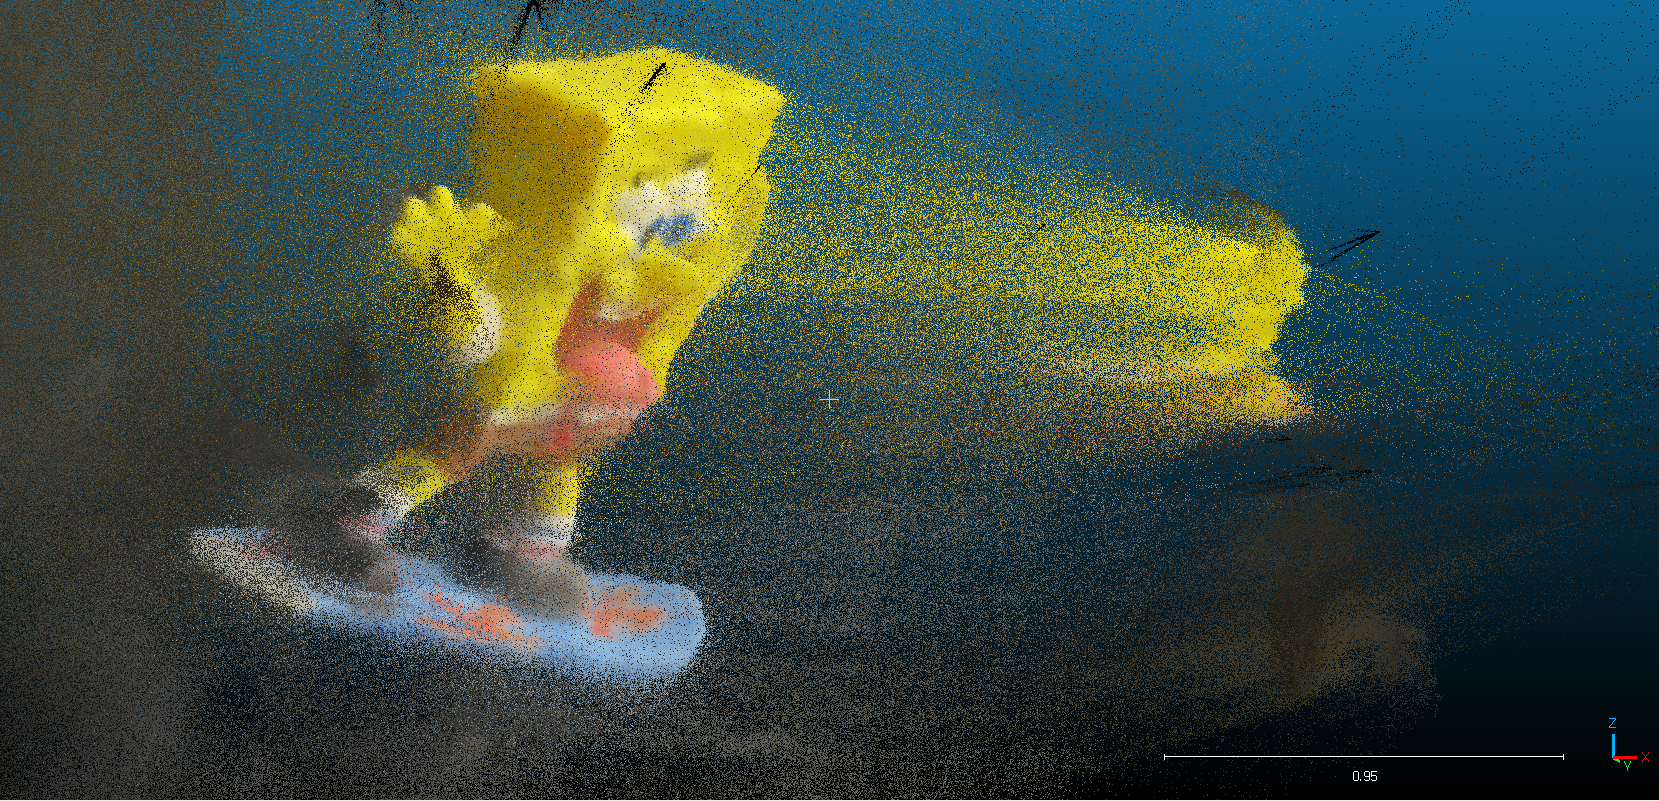
\includegraphics[width=0.8\textwidth]{../images/230724/pc3.png}}\hfill
    \caption{InfoNeRF Results point cloud with dropout 10000iteration}
    \label{fig:dropout_pc}
\end{figure}

\newpage


실험결과\ref{fig:dropout_pc}는 위와 같다. 더욱 아래 보드 부분은 더욱 군집이 잘 형성되었지만 
spongebob에 얼굴 부분이 두 부분으로 나누어진 것이 확인가능하다. 
실험을 진행함에 있어 적절한 early,late dropout을 찾는 과정에는 여러 차례의 실험이 필요하다.
해당 결과에 경우 실험없이 나온 결과이기 때문에, 더욱 많은 실험을 해봐야 결론을 내릴 수 있을것으로 생각된다. 

\begin{figure}[h]
    \centering
    
    \subfloat[rendered scene]{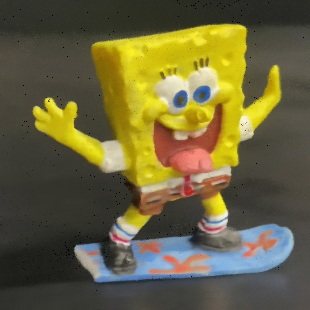
\includegraphics[width=0.25\textwidth]{../images/230724/dropout/000.png}}\hfill
    \subfloat[rendered scene]{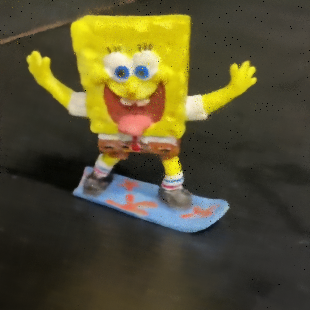
\includegraphics[width=0.25\textwidth]{../images/230724/dropout/001.png}}\hfill
    \subfloat[rendered scene]{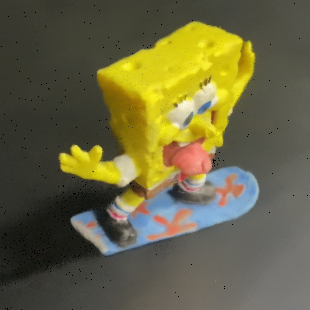
\includegraphics[width=0.25\textwidth]{../images/230724/dropout/002.png}}\hfill
    \subfloat[rendered scene]{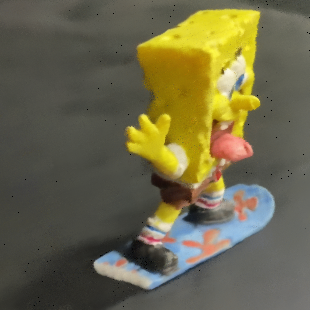
\includegraphics[width=0.25\textwidth]{../images/230724/dropout/003.png}}\hfill
    \subfloat[rendered scene]{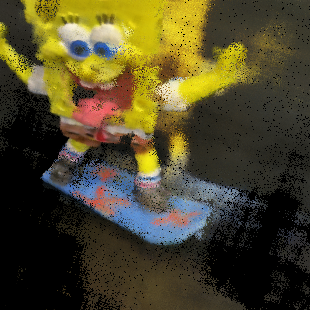
\includegraphics[width=0.25\textwidth]{../images/230724/dropout/004.png}}\hfill
    \subfloat[rendered scene]{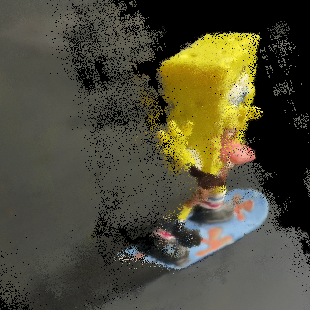
\includegraphics[width=0.25\textwidth]{../images/230724/dropout/005.png}}\hfill
    \subfloat[rendered scene]{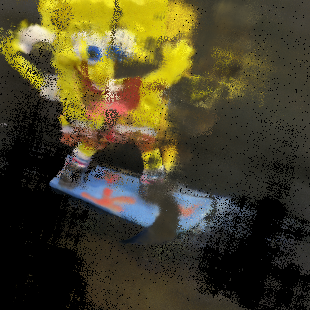
\includegraphics[width=0.25\textwidth]{../images/230724/dropout/012.png}}\hfill
    \subfloat[rendered scene]{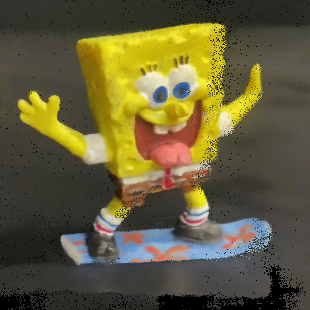
\includegraphics[width=0.25\textwidth]{../images/230724/dropout/018.png}}\hfill
    \subfloat[rendered scene]{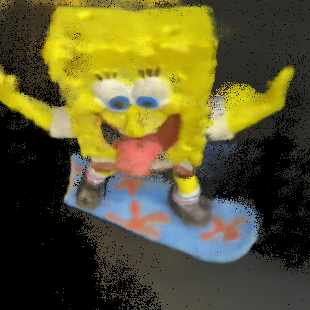
\includegraphics[width=0.25\textwidth]{../images/230724/dropout/023.png}}\hfill
    \subfloat[rendered scene]{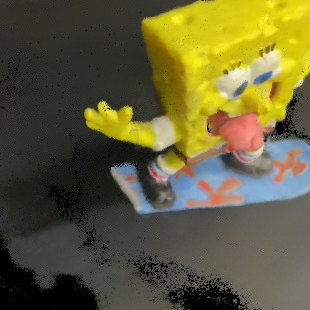
\includegraphics[width=0.25\textwidth]{../images/230724/dropout/032.png}}\hfill
    \subfloat[rendered scene]{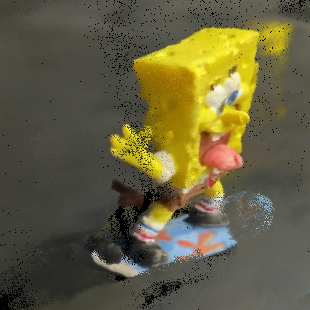
\includegraphics[width=0.25\textwidth]{../images/230724/dropout/044.png}}\hfill
    \subfloat[rendered scene]{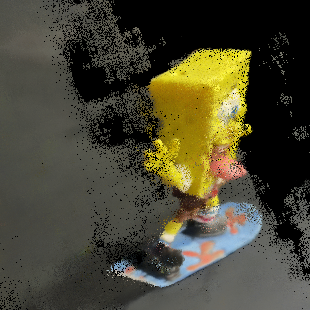
\includegraphics[width=0.25\textwidth]{../images/230724/dropout/051.png}}\hfill

    
    \caption{InfoNeRF Results rendered image with dropout}
    \label{fig:dropout_rendered}
\end{figure}

\newpage


\subsection{encoding 개선}

Pixel NeRF\cite{pixelnerf}에서 아이디어를 얻어 segmentation map을 이용하여 MLP에 추가 input을 추가하는 구조를 고안해봤다.
pixelnerf는 \ref{fig:pixelnerf} 과 같은 구조를 같는다 기존 nerf와 다르게 scene간에 prior infomation을 학습시켜
적은 장면만으로도 3d scene reconstruction이 가능하도록한다. 

\newpage


\begin{figure}[h]
    \centering
    \subfloat[Pixel NeRF flow]{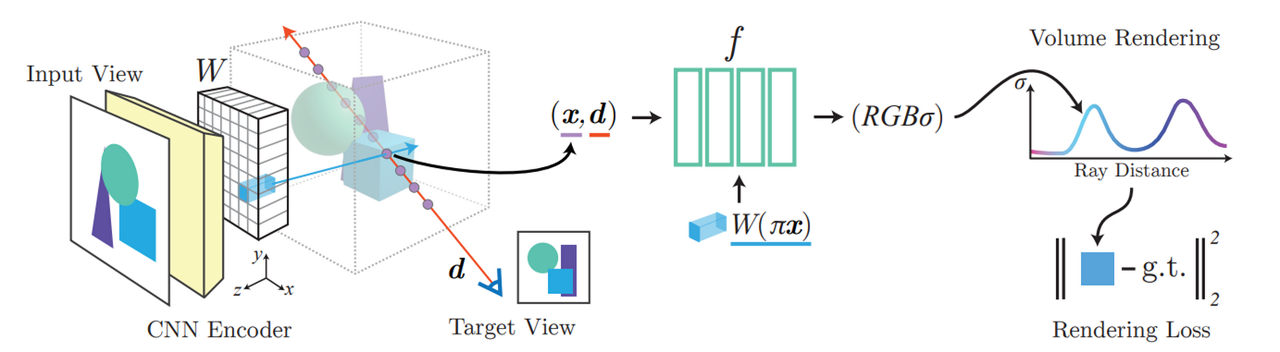
\includegraphics[width=0.8\textwidth]{../images/230724/pixelnerf.png}}\hfill
    \subfloat[Pixel NeRF layor]{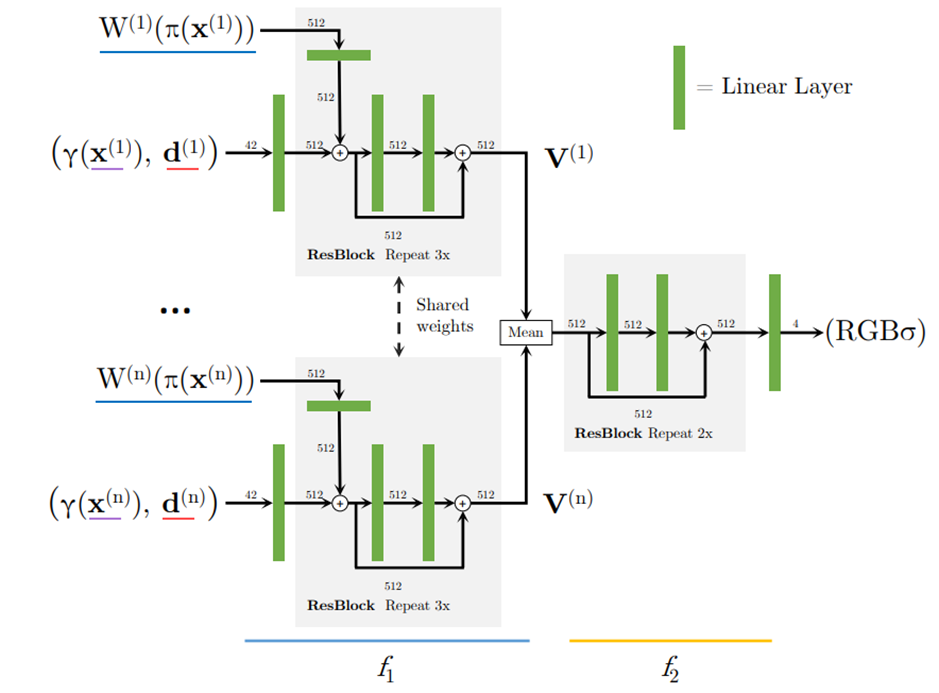
\includegraphics[width=0.8\textwidth]{../images/230724/pixelnerf2.png}}\hfill
    \caption{Pixel NeRF overview}
    \label{fig:pixelnerf}
\end{figure}

해당 구조에 착안하여 prior infomation을 사용한 nerf를 사용하기 위해 
pixelnerf에 인코더 대신 segmentation map을 추가적인 input으로 받는 nerf를 구상해보았다.

\begin{figure}[h]
    \centering
    \subfloat[segmentation map1]{
\includegraphics[width=0.25\textwidth]{../images/230724/s_0.png}}\hfill
    \subfloat[segmentation map2]{
\includegraphics[width=0.25\textwidth]{../images/230724/s_100.png}}\hfill
    \subfloat[segmentation map3]{
\includegraphics[width=0.25\textwidth]{../images/230724/s_235.png}}\hfill
    \subfloat[segmentation map4]{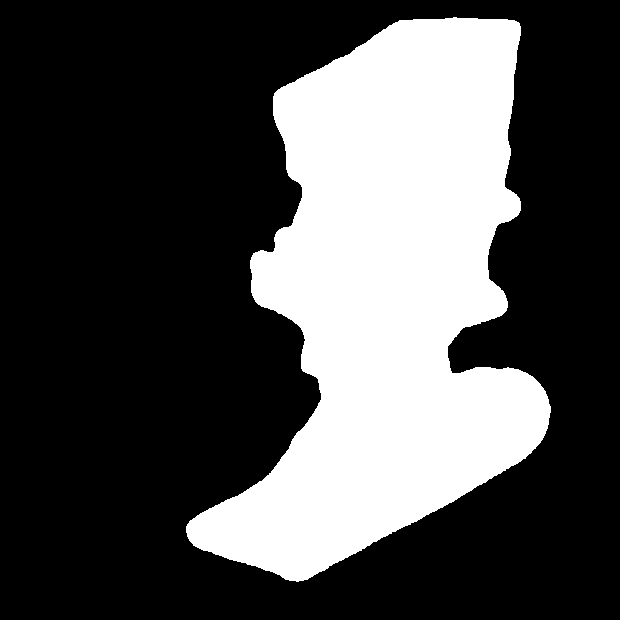
\includegraphics[width=0.25\textwidth]{../images/230724/s_340.png}}\hfill
    \caption{segmentation map}
    \label{fig:pixelnerf}
\end{figure}
\newpage

해당 정보들을 pixelnerf에 encoding의 결과로 나온 feature vector처럼 사용할 예정이다.

\newpage

\section*{Action items in next week}	%% Action items in next week
다음 주에는 
\begin{enumerate}
    \item 세미나 준비
    \item U-surf 활동 마무리 
\end{enumerate}
등을 진행하도록 하겠습니다.

\bibliographystyle{IEEEtran} 
\bibliography{refer} 
\end{document}